\documentclass[a4paper,oneside,11pt]{report}

% Packages laden
\usepackage[a4paper,top=2cm,bottom=2cm,left=3cm,right=2cm]{geometry}		% paginagrootte
\usepackage{parskip}					% andere regels voor nieuwe paragraaf: witregel + niet inspringen

\usepackage[latin1]{inputenc}					% invoer van speciale tekens (bvb. Umlaut)
\usepackage{lmodern}						% betere weergave van speciale tekens (bvb. Umlaut)
\usepackage{dsfont}	
\usepackage{amsfonts,amsthm, tabularx}			% wiskundige symbolen and table of equations
%\usepackage{mathtools}
\usepackage{enumerate}

\usepackage{graphicx,subcaption}					% figuren
\usepackage{float}								% plaatsen van figuren en tabellen
\usepackage[font=small,labelfont=bf]{caption}
\usepackage[format=plain,indent=1cm]{caption}
\usepackage{eurosym}
\usepackage[squaren,Gray]{SIunits}
\usepackage{amsmath,amsfonts,amsthm,mathrsfs,MnSymbol}	% wiskundige symbolen
\usepackage{pifont}	
\usepackage{color}				% Load the color package: \color{declared-color}{text}. If also background:
								% \colorbox{declared-color1}{\color{declared-color2}text}
\usepackage[dutch]{babel}		% spellingcorrectie Nederlands
\usepackage{titling}
\usepackage{epstopdf}
\usepackage{stackengine}
\usepackage{graphicx}
\usepackage{hyperref}

\graphicspath{{./Figures/}}
	% personaliseren van onderschriften
\captionsetup[table]{name=Tabel}
							% sign of euro


% Instellingen voor document
\renewcommand{\arraystretch}{1.1}				% tabelrijen iets hoger maken
\urlstyle{same}
\hypersetup{hidelinks=true}

\renewcommand*\thesection{\arabic{section}}
\DeclareMathOperator*{\argmin}{\arg\!\min}

\numberwithin{figure}{section}
\numberwithin{table}{section}
\numberwithin{equation}{section}					

\setcounter{secnumdepth}{3}		% Enable subsubsection numbering
\setcounter{tocdepth}{3}		% Include subsubsection in table of content

\pagenumbering{arabic}

\begin{document}
%\pagenumbering{gobble}
\newpage


\section{Definitie}

De meest algemene definitie van de ladingstoestand (SoC) is de verhouding tussen de huidige energie-inhoud $E(t)$ en de maximale energie-inhoud $E_{max}$ die een boorveld kan bezitten. \cite{R28}
\\ \begin{equation}\label{def_eq1}
SoC=\dfrac{E(t)}{E_{max}}
\end{equation}

In de diepte bestaat een boorveld uit verschillende lagen aangezien de bodemeigenschappen van de verschillende bodemlagen sterk kunnen verschillen. Stel nu dat het boorveld bestaat uit N lagen, dan kan voor elke laag n de ladingstoestand, $SoC_n$ opgesteld worden. De totale ladingstoestand, $SoC_{tot}$, volgt dan uit deze individuele ladingstoestanden. Figuur \ref{fig:def_1} toont de doorsnede van een U-boorveld met 2 lagen. 

\begin{figure}[hbtp] 
	\centering
	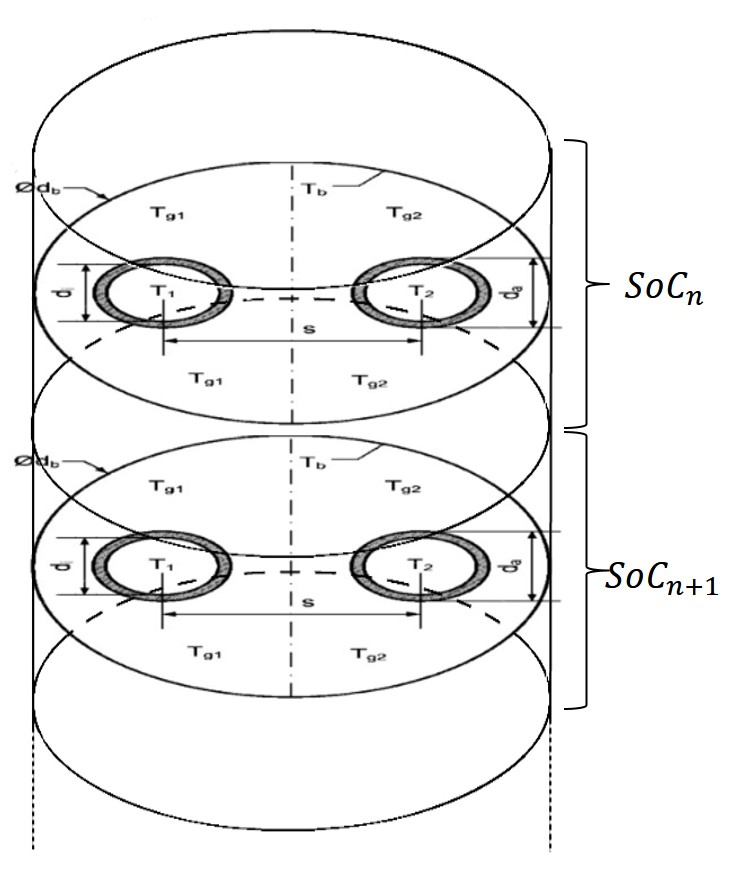
\includegraphics[width=0.4 \textwidth]{def_fig1.jpg}
	\caption{Doorsnede van een U-boorveld met 2 lagen.}
	\label{fig:def_1}
\end{figure}
 

Door gebruik te maken van thermische weerstanden en thermische warmtecapaciteiten, kan per laag een equivalent schema opgesteld worden, zoals getoond in Figuur \ref{fig:def_2} en Figuur \ref{fig:def_3} \cite{R23}. Met behulp van dit equivalent schema is de definitie voor de ladingstoestand van laag n, $SoC_n$,  de volgende.\cite{R28}\\
\begin{equation}\label{def_eq2}
SoC_n=\dfrac{\sum\limits_{i=1}^k m_{i,n}.c_{p_{i,n}}.(T_{i,n}(t)-T_{n,ref})}{\sum\limits_{i=1}^k m_{i,n}.c_{p_{i,n}}.(T_{i,n,max}-T_{n,ref})}
\end{equation}
Hieruit volgt dan ook de definitie van de totale ladingstoestand, $SoC_{tot}$ door te sommeren over de verschillende lagen.
\\
\begin{equation}\label{def_eq3}
SoC_{tot}=\dfrac{\sum\limits_{n=1}^N \sum\limits_{i=1}^k m_{i,n}.c_{p_{i,n}}.(T_{i,n}(t)-T_{n,ref}) }{\sum\limits_{n=1}^N \sum\limits_{i=1}^k m_{i,n}.c_{p_{i,n}}.(T_{i,n,max}-T_{n,ref})}
\end{equation}

\begin{figure}[hbtp] 
	\centering
	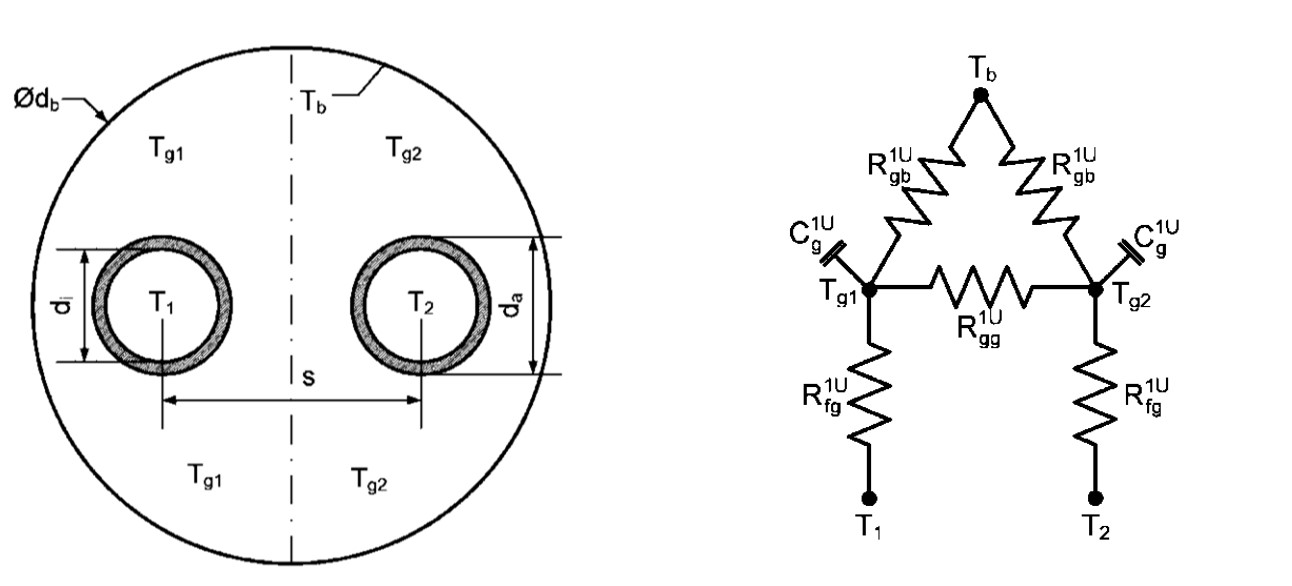
\includegraphics[width=0.8 \textwidth]{def_fig2.jpg}
	\caption{Equivalent schema van \'e\'en laag.}
	\label{fig:def_2}
\end{figure}

\begin{figure}[hbtp] 
	\centering
	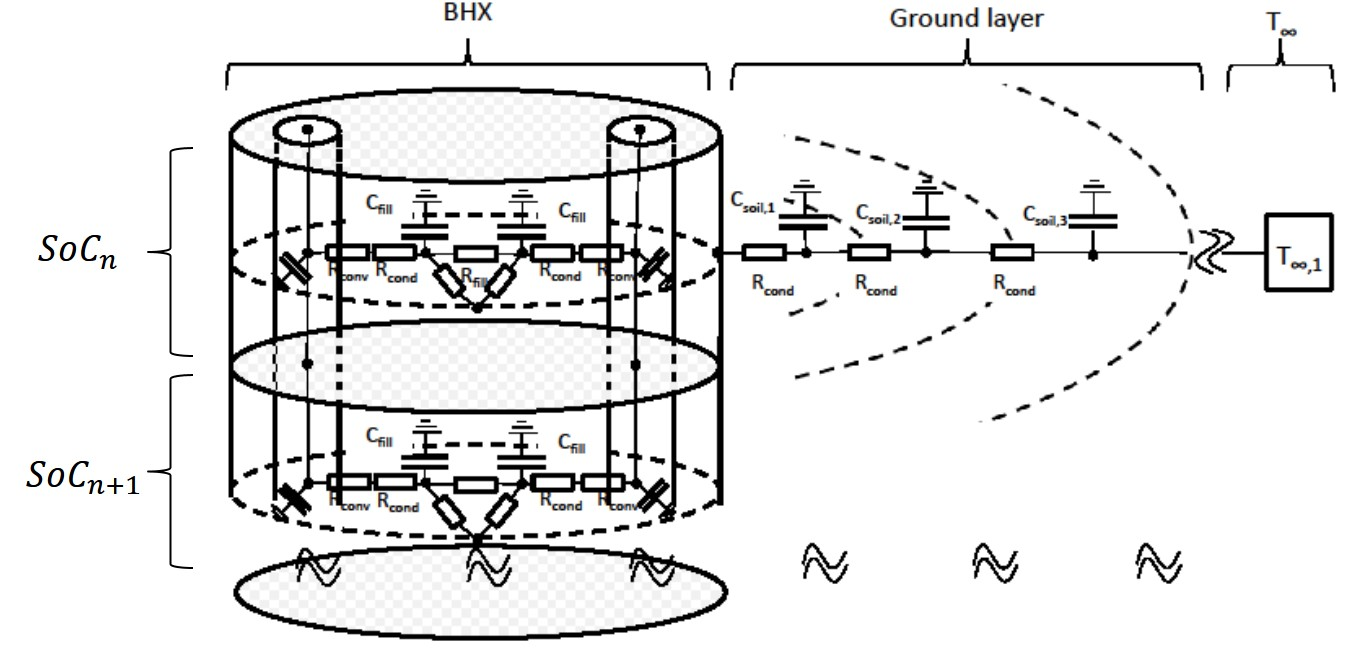
\includegraphics[width=0.8 \textwidth]{def_fig3.jpg}
	\caption{Weergave van het equivalent schema voor verschillende lagen.}
	\label{fig:def_3}
\end{figure}


\textcolor{red}{In Modelica bibliotheek "IDEAS" is er een model beschikbaar dat zowel korte termijn als lange termijn combineert (Damien Picard en Prof. Helsen) \cite{R7}, \cite{R25}.} 
  


Een belangrijke input in dit model is de referentietemperatuur. Een eerste mogelijke keuze is het gebruiken van de wettelijke temperatuurslimiet. Deze wettelijke limiet ligt in Belgi\"e op een minimum van 0 \degree C en een maximum van 25 \degree C \cite{}. Bij deze keuze behaalt de ladingstoestand waarschijnlijk nooit een waarde van 0 of 1 aangezien de temperatuur deze limieten niet bereikt. 
Een tweede optie bestaat erin om de technische limieten te gebruiken. Bijvoorbeeld voor koeling van een gebouw moet de grondtemperatuur lager blijven dan de temperatuur die nodig is om de ruimte te koelen. Maar tegelijkertijd moet de grondtemperatuur ook hoger zijn dan de vriestemperatuur van het koelmiddel. 
\begin{equation} \label{def_eq4}
T_{vries}<T_{grond}<T_{aanvoer,koeling}
\end{equation}
Analoog voor de verwarming van een gebouw.
\begin{equation}\label{def_eq5}
T_{aanvoer,verwarming}<T_{grond}<T_{kook}
\end{equation}
Om de grootste range, van waarde 0 tot 1, van de ladingstoestand te behalen is het nuttig om de werkelijke gebruikslimieten te gebruiken. Deze werkelijke gebruikslimieten kunnen veranderlijk zijn in de tijd. 

\newpage
\section{Invloedsfactoren}
Om een gepast model op te stellen, is het belangrijk de invloed van parameters en eigenschappen te kennen en welke nauwelijks invloed hebben. Belangrijk hierbij op de merken is dat de bepaling van deze parameters en eigenschappen mogelijk moet zijn, ofwel enerzijds door metingen uit te voeren of door databanken te raadplegen. 
\textcolor{red}{De gegevens moeten ook bruikbaar zijn in een regelaar.}
\par Een opsomming van de mogelijke invloedsfactoren op de ladingstoestand staat hieronder. De factoren met de grootste invloed op de ladingstoestand, onderstreept in onderstaande lijst, worden verder toegelicht. 
\begin{itemize}
\item Bodemeigenschappen
	\begin{itemize}
	\item Bodemstructuur en materiaal van de bodem
   	\item \underline{Thermische conductiviteit} ($k$)
	\item \underline{Thermische diffusiviteit} ($\alpha$)
	\item \underline{Volumetrische warmtecapaciteit} ($c$)
	\item Porositeit ($\varphi$)
	\end{itemize}	
\item Temperatuur
	\begin{itemize}
	\item \underline{Temperatuur aan grondoppervlak}
	\end{itemize}
\item \underline{Grondwaterstroming}
\item Dimensies
	\begin{itemize}
	\item Lengte van het boorgat
	\item \underline{Lay-out van het boorgatenergieopslagveld}
	\end{itemize}
\item \underline{Bodemsaturatie}
\end{itemize}
	

\subsection*{Thermische conductiviteit, diffusiviteit en warmtecapaciteit}
De thermische conductiviteit $k$, thermische diffusiviteit $\alpha$ en de volumetrische warmtecapaciteit $c$ zijn gelinkt via volgende relatie.
\begin{equation}\label{invlf_eq1}
\alpha=\dfrac{k}{\rho.c_p}=\dfrac{k}{c}
\end{equation}
De meest geschikte toepassing van het energieopslagveld is afhankelijk van de thermische conductiviteit. Bij een grote thermische conductiviteit, regenereert de bodem snel. De bodem is dan het meest geschikt als een dissipator van energie. Dit is zo als de warmtevraag ongebalanceerd is, enkel een warmtevraag of koudevraag gedurende het hele jaar. Is de thermische conductiviteit klein, dan is de bodem geschikt als energieopslag. De warmtevraag dient dan gebalanceerd te zijn. Gedurende het jaar is er vraag naar warmte en koeling.
\par Smart Geotherm stelt geschiktheidskaarten ter beschikking. Er zijn kaarten verkrijgbaar voor de gemiddelde thermische conductiviteit (Figuur \ref{fig:invlf_1}), de maximale gemiddelde thermische conductiviteit (Figuur \ref{fig:invlf_2}) en de minimale gemiddelde thermische conductiviteit (Figuur \ref{fig:invlf_3}) voor een diepte van 100 m of tot de diepte van een vaste rots \cite{}. De gemiddelde thermische conductiviteit bepaalt meestal de meest geschikte toepassing. Sectie \ref{}  behandelt de invloed van het gebruik van de gemiddelde, maximale of minimale thermische conductiviteit op de ladingstoestand. 

\textcolor{red}{Tekst toevoegen: Vereenvoudiging lagen door equivalente parameters.}

\begin{figure}[hbtp] 
	\centering
	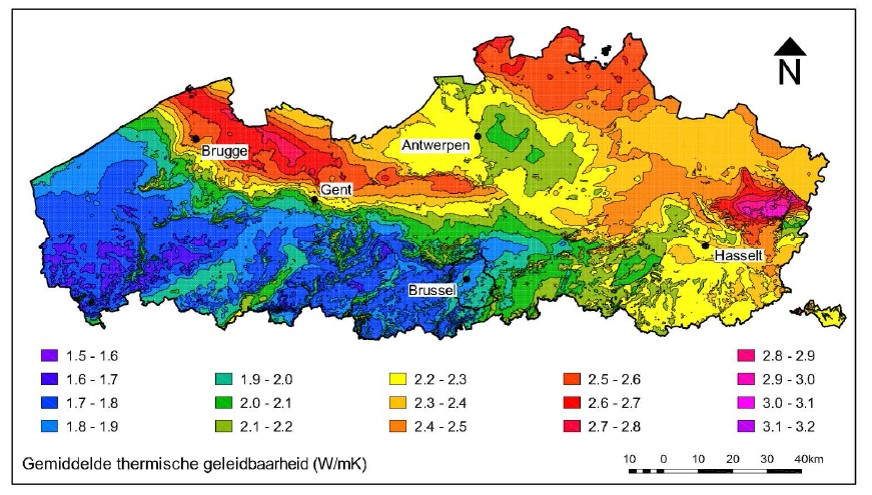
\includegraphics[width=0.7 \textwidth]{invlf_fig1.jpg}
	\caption{Gemiddelde thermische geleidbaarheid tot op een diepte van 100 m of tot op de vaste rots.}
	\label{fig:invlf_1}
\end{figure}

\begin{figure}[hbtp] 
	\centering
	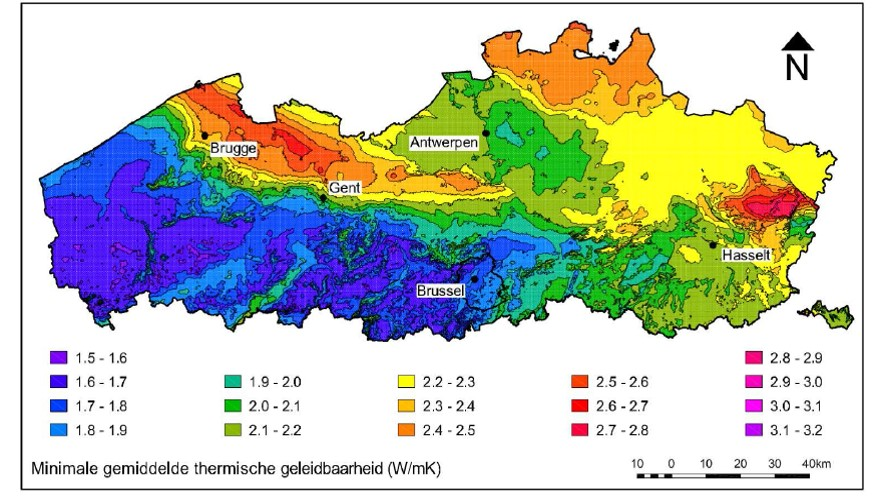
\includegraphics[width=0.7 \textwidth]{invlf_fig2.jpg}
	\caption{Minimale gemiddelde thermische geleidbaarheid tot op een diepte van 100 m of tot op de vaste rots.}
	\label{fig:invlf_2}
\end{figure}

\begin{figure}[hbtp] 
	\centering
	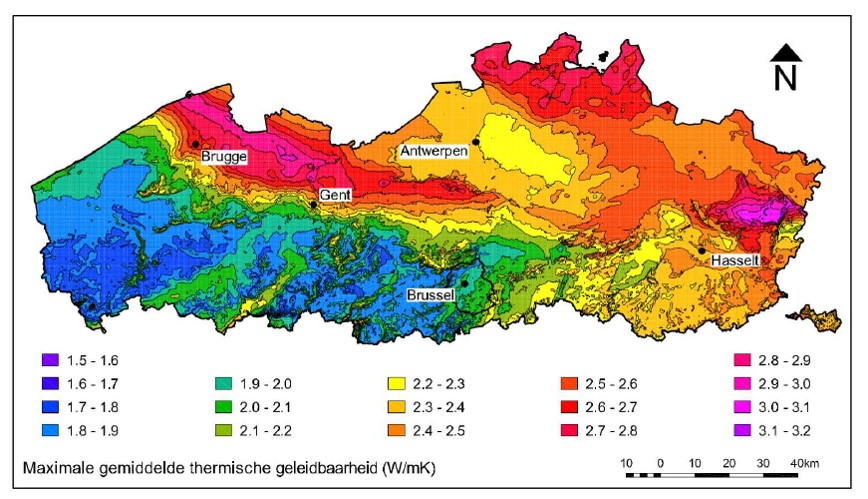
\includegraphics[width=0.7 \textwidth]{invlf_fig3.jpg}
	\caption{Maximale gemiddelde thermische geleidbaarheid tot op een diepte van 100 m of tot op de vaste rots.}
	\label{fig:invlf_3}
\end{figure}


\subsection*{Temperatuur van grondoppervlak}
Vooral de bovenste lagen van de bodem ondervinden een invloed van de buitentemperatuur aan het grondoppervlak. Figuur \ref{fig:invlf_4} geeft dit temperatuursverloop weer. Vanaf een diepte van 10 \'a 30 m is de temperatuur nagenoeg constant (10 - 12 \degree C). Hierna stijgt de temperatuur met 3 \degree C per 100 m \cite{}. Indien deze eerste 10 \'a 30 m relatief een significant deel vormt van de diepte van het boorgat, dient dit temperatuursverloop in rekening gebracht te worden. 
 
\begin{figure}[hbtp] 
	\centering
	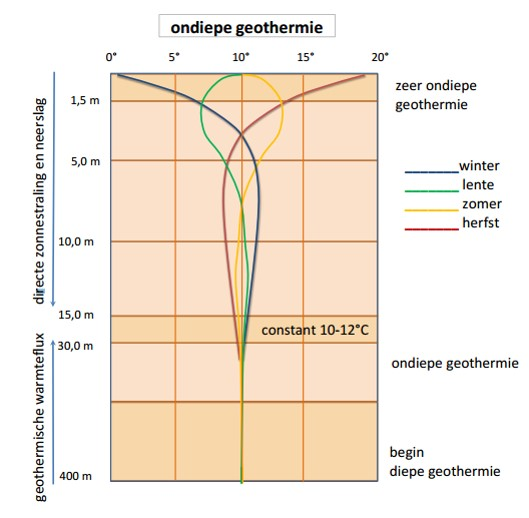
\includegraphics[width=0.45 \textwidth]{invlf_fig4.jpg}
	\caption{Temperatuursverloop in functie van de diepte.}
	\label{fig:invlf_4}
\end{figure}

\subsection*{Grondwaterstroming}
De eventuele aanwezigheid van grondwaterstroming heeft een invloed op de temperatuurverdeling rondom het boorveld. Indien de temperatuurverdeling niet meer symmetrisch is rondom het boorgatenergieopslagveld heeft dit een invloed op de modellering. Grondwaterstroming zorgt ervoor dat de bodem sneller regenereert waardoor het geschikt is voor energiedissipatie.
Een karakteristiek getal voor grondwaterstroming is het P\'eclet-getal \cite{}. 
\begin{equation} \label{invlf_eq2}
Pe=\dfrac{r_b.v}{\alpha}=\dfrac{r_b.\Phi}{\alpha.\varphi}
\end{equation}
Hierbij is $v$ niet de snelheid waarmee de vloeistof door de pori\"en stroomt, maar wel de Darcysnelheid. Slechts een fractie van het volume is echter beschikbaar voor stroming. 

\subsection*{Lay-out}
De lay-out van een boorveld kan een lijn of een meer compacte vorm, een matrix vorm, zijn. (Figuur 7) Samen met de eventuele aanwezigheid van grondwaterstroming heeft de lay-out een sterke invloed op de temperatuurverdeling, op het temperatuursverloop in de tijd, alsook de tijd om een evenwichtstoestand te bereiken en op de effici\"entie van het boorgatenergieopslagveld. Ook het feit of de vraag gebalanceerd of ongebalanceerd is speelt een rol.
\par Bij volgende simulaties werd de invloed van de temperatuur van het grondoppervlak verwaarloosd \cite{R10}. Voor een gebalanceerde vraag met grondwaterstroming heeft grondwaterstroming nauwelijks effect, ongeacht de lay-out. Indien de vraag daarentegen ongebalanceerd is, kan dit een sterke invloed hebben op het temperatuursverloop \cite{R10}. (Figuur 8)
\par Bij een ongebalanceerde vraag is de invloed van grondwaterstroming significant. Het koudste punt van de temperatuurverdeling verplaatst zich stroomafwaarts buiten het middelpunt van de matrix lay-out. Figuur \ref{fig:invlf_7} geeft de temperatuurverdeling van een boorgatenergieopslagveld met matrix lay-out weer\cite{R10}. 
\par De invloed van de lay-out bij een ongebalanceerde warmtevraag en zonder grondwaterstroming is weergegeven in Figuur \ref{fig_invlf_8}. Hierbij dient aandacht besteed te worden aan de afstandsschaal. 10 m buiten het middelpunt bij de matrix lay-out bereikt de grond gemiddeld een temperatuur van 4 \degree C. Bij de lijn lay-out is de temperatuur 10 m buiten de lijn 8 \degree C. Dit is een significant verschil \cite{R10}.
\par \textcolor{red}{De effici\"entie van een boorveld daalt bij een vierkante lay-out. Dit hangt ook sterk samen met een gebalanceerde, warmte en koudevraag, of een ongebalanceerde warmtevraag. }

\begin{figure}[hbtp] 
\begin{subfigure}{0.3\textwidth}
	\centering
	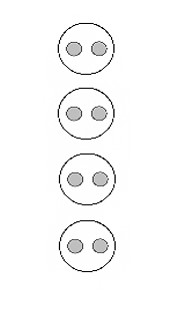
\includegraphics[height=0.95\textwidth]{invlf_fig5a.jpg}
	\caption{Lijn lay-out}
\end{subfigure}%
\begin{subfigure}{0.3\textwidth}
	\centering
	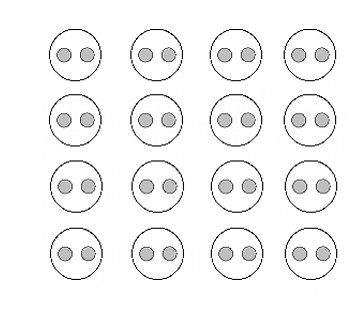
\includegraphics[height=0.95\textwidth]{invlf_fig5b.jpg}
	\caption{Matrix lay-out}
\end{subfigure}
\label{fig:invlf_5}
\centering
\caption{Mogelijke lay-outs van een boorgatenergieopslagveld.}
\end{figure}

\begin{figure}[hbtp] 
\begin{subfigure}{0.75\textwidth}
	\centering
	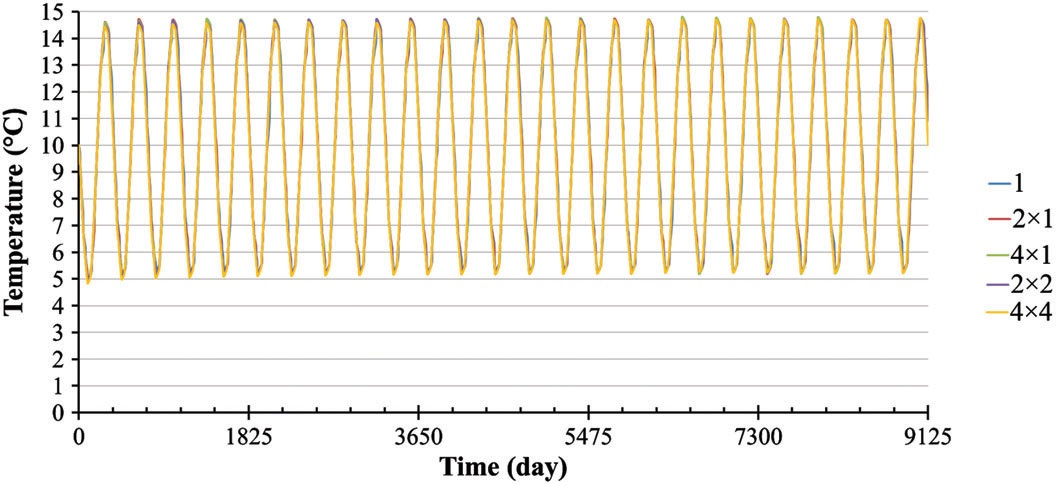
\includegraphics[width=0.75\textwidth]{invlf_fig6a.jpg}
	\caption{Gebalanceerde vraag met grondwaterstroming.}
\end{subfigure}
\begin{subfigure}{0.75\textwidth}
	\centering
	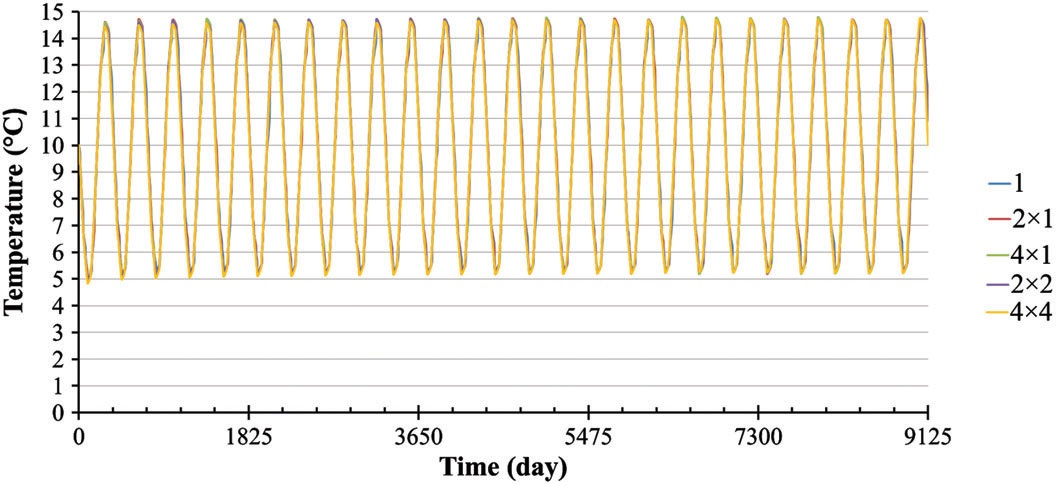
\includegraphics[width=0.75\textwidth]{invlf_fig6a.jpg}
	\caption{Ongebalanceerde vraag met grondwaterstroming.}
\end{subfigure}
\label{fig:invlf_6}
\centering
\caption{De grondtemperatuur doorheen de tijd.}
\end{figure}

\begin{figure}[hbtp] 
\begin{subfigure}{0.4\textwidth}
	\centering
	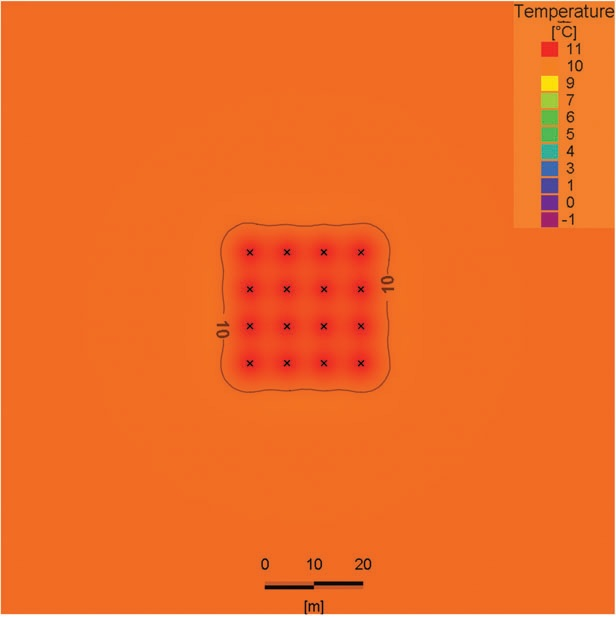
\includegraphics[width=0.95\textwidth]{invlf_fig7a.jpg}
	\caption[width=0.95\textwidth]{Gebalanceerde vraag zonder grondwaterstroming.}
\end{subfigure}%
\begin{subfigure}{0.4\textwidth}
	\centering
	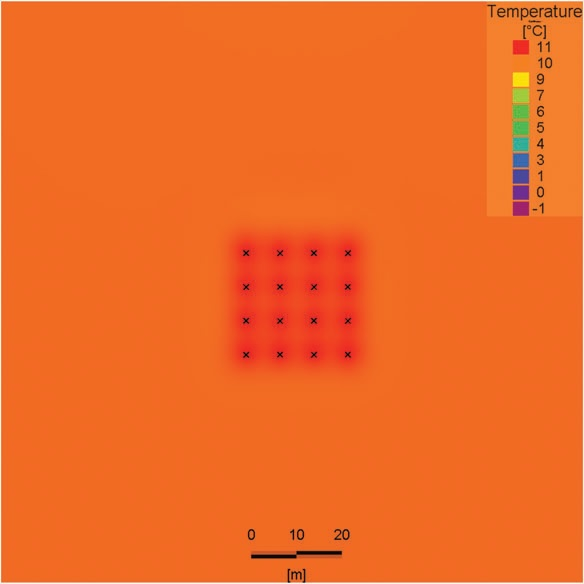
\includegraphics[width=0.95\textwidth]{invlf_fig7b.jpg}
	\caption[width=0.95\textwidth]{Gebalanceerde vraag met grondwaterstroming.}
\end{subfigure}
\begin{subfigure}{0.4\textwidth}
	\centering
	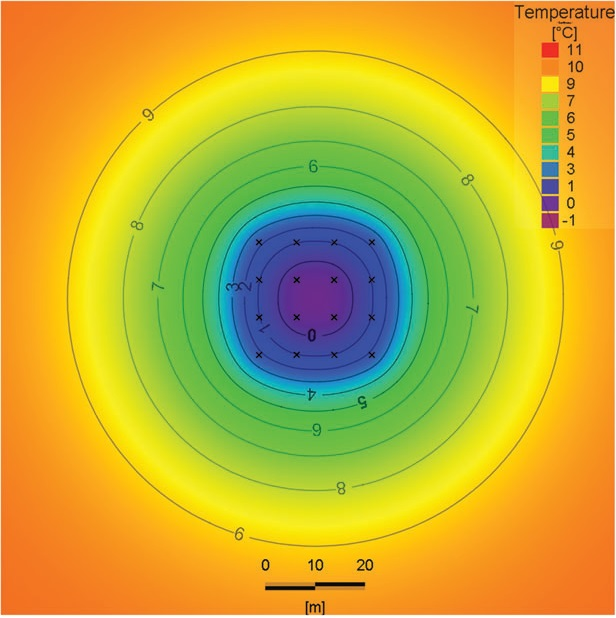
\includegraphics[width=0.95\textwidth]{invlf_fig7c.jpg}
	\caption[width=0.95\textwidth]{Ongebalanceerde vraag zonder grondwaterstroming.}
\end{subfigure}%
\begin{subfigure}{0.4\textwidth}
	\centering
	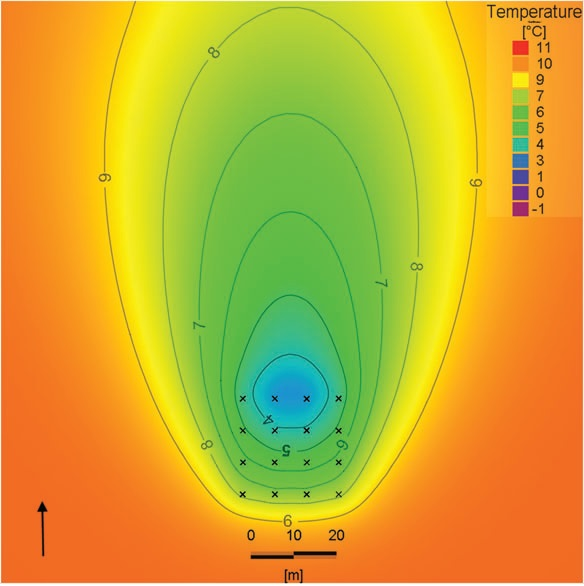
\includegraphics[width=0.95\textwidth]{invlf_fig7d.jpg}
	\caption[width=0.95\textwidth]{Ongebalanceerde vraag met grondwaterstroming.}
\end{subfigure}%
\label{fig:invlf_7}
\centering
\caption{De temperatuursverdeling van een boorgatenergieopslagveld met matrix lay-out in verschillende situaties van vraag en grondwaterstroming.}
\end{figure}

\begin{figure}[hbtp] 
\begin{subfigure}{0.4\textwidth}
	\centering
	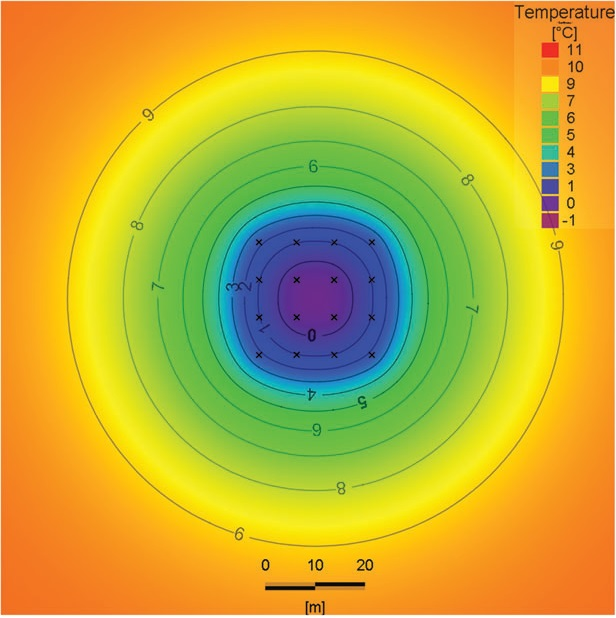
\includegraphics[width=0.95\textwidth]{invlf_fig8a.jpg}
	\caption{Matrix lay-out.}
\end{subfigure}%
\begin{subfigure}{0.4\textwidth}
	\centering
	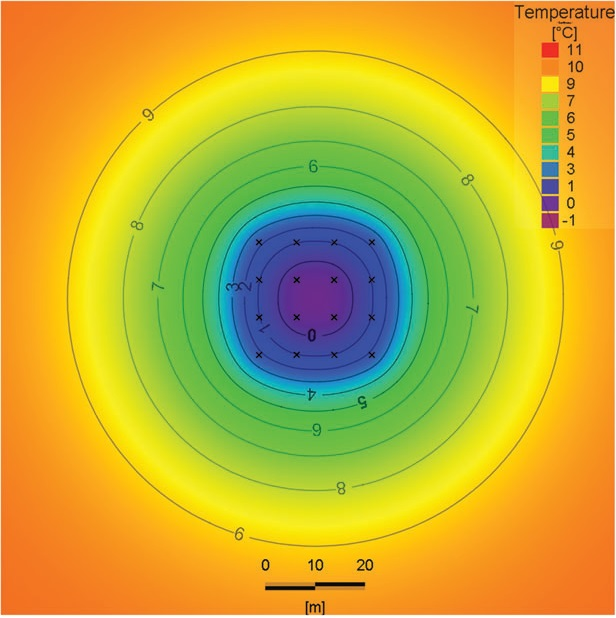
\includegraphics[width=0.95\textwidth]{invlf_fig8a.jpg}
	\caption{Lijn lay-out.}
\end{subfigure}%
\label{fig:invlf_8}
\centering
\caption{De temperatuursverdeling van een boorgatenergieopslagveld bij verschillende lay-outs met een ongebalanceerde warmtevraag en zonder grondwaterstroming.}
\end{figure}


\subsection*{Bodemsaturatie}
De graad van bodemsaturatie $S$ geeft de waterinhoud van de bodem weer. De waarde van $S$ ligt tussen 0 en de porositeit $\varphi$. 
\begin{equation}\label{invlf_eq3}
S=\dfrac{V_{water}}{V_{water}+v_{lucht}+V_{materiaal}}
\end{equation}
De bodemsaturatie is afhankelijk van de locatie in het boorgatenergieopslagveld. Bij een stijgende graad van saturatie, stijgt de thermische conductiviteit $k$ alsook de thermische diffusiviteit $\alpha$. Aangezien de bodemsaturatie ook verandert in de tijd, zijn de thermische conductiviteit en thermische diffusiviteit ook tijdsafhankelijk \cite{R2}.

\textcolor{red}{Figuur invoegen}

% Na de bijlagen plaatst men nog de bibliografie.
% Je kan de  standaard "abbrv" bibliografiestijl vervangen door een andere.
\bibliographystyle{abbrv}
\bibliography{referenties}


\end{document}
